\chapter{问题回顾}
\label{cha:question}

\section{问题重述}
%content
%research current state here
2017年8月8日,四川阿坝州九寨沟县发生7.0级地震,造成了不可挽回的人员伤亡和重大的财产损失。由于预测地震比较困难,及时高效的灾后救援是减少地震损失的重要措施。无人机作为一种新型运载工具,能够在救援行动中发挥重要作用。为提高其使用效率,请你们解决无人机优化运用的几个问题。
附件1给出了震区的高程数据,共有2913列,2775行。第一行第一列表示(0,0)点处的海拔高度值(单位:米),相邻单元格之间的距离为38.2米,即第m行第n列单元格中的数据代表坐标(38.2(m-1), 38.2(n-1))处的高度值。震区7个重点区域的中心位置如下表所示(单位:千米):
\begin{table}
\centering
\begin{tabular}{|c|c|c|}
\hline
中心点&X坐标&Y坐标\\
\hline
A&30.3&89.8\\
\hline
B&66.0&84.7\\
\hline
C&98.4&76.7\\
\hline
D&73.7&61.0\\
\hline
E&57.9&47.6\\
\hline
F&86.8&22.0\\
\hline
G&93.6&48.8\\
\hline
\end{tabular}
\end{table}
除另有说明外,本题中的无人机都假设平均飞行速度60千米/小时,最大续航时间为8小时,飞行时的转弯半径不小于100米,最大爬升(俯冲)角度为±15°,与其它障碍物(含地面)的安全飞行距离不小于50米,最大飞行高度为海拔5000米。所有无人机均按规划好的航路自主飞行,无须人工控制,完成任务后自动返回原基地。
\subsection{问题一:灾情巡查}
大地震发生后,及时了解灾区情况是制订救援方案的重要前提。为此,使用无人机携带视频采集装置巡查7个重点区域中心方圆10公里(并集记为S)以内的灾情。假设无人机飞行高度恒为4200米,将在地面某点看无人机的仰角大于60°且视线不被山体阻隔视为该点被巡查。若所有无人机均从基地H(110,0)(单位:千米)处派出,且完成任务后再回到H,希望在4小时之内使区域S内海拔3000米以下的地方尽可能多地被巡查到,最少需要多少架无人机?覆盖率是多少?每架无人机的飞行路线应如何设计?在论文中画出相应的飞行路线图及巡查到的区域(不同的无人机的飞行路线图用不同的颜色表示)。

进一步,为及时发现次生灾害,使用无人机在附件1给出的高度低于4000米的区域(不限于S)上空巡逻。问最少需要多少架无人机、如何设定每架无人机的飞行时间、路线,才能保证在72小时内,上述被巡查到的地方相邻两次被巡查的时间间隔不大于3小时(无人机均需从H出发并在8小时内回到H,再出发的时间间隔不小于1小时)?
\begin{figure}[!ht]
\centering
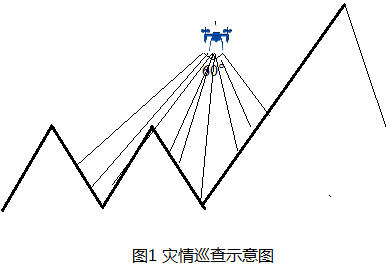
\includegraphics[width=6cm]{problem_1.png}
\end{figure}
\subsection{问题二:生命迹象探测}
使用无人机携带生命探测仪搜索生命迹象,能够给灾后救援提供准确的目标定位。拟从基地H(110,0),J(110,55)(单位:千米)处总共派出30架无人机(各15架),任务完成后回到各自的出发地。探测仪的有效探测距离不超过1000米,且最大侧视角(探测仪到可探测处的连线与铅垂线之间的夹角)为60度。请你们规划它们的飞行路线,使附件1所给出的全区域内海拔3000米以下部分能被探测到的面积尽可能大,且使从第一架无人机飞出到最后一架完成任务的无人机回到基地的时间间隔尽量短。
\begin{figure}[!ht]
\centering
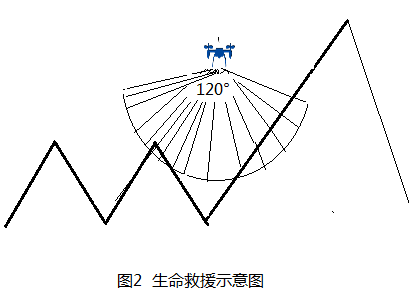
\includegraphics[width=6cm]{problem_2.png}
\end{figure}
\subsection{问题三:灾区通信中继}
大地震发生后,地面电力设施被破坏,灾区通信中断。太阳能无人机(白天不受续航能力限制,其余条件同前述)
可以作为地面移动终端之间的通信中继,为灾区提供持续的通信保障(地面终端只能与无人机进行通信,
无人机之间只要不超过最大通信距离就可以互相通信,地面与地面之间的通信由无人机转接)。
假设无人机在空中飞行时,可与距离3000米以内的移动终端通信,无人机之间的最大通信距离为6000米,
问最少需要多少架无人机、每架无人机的飞行路线如何,才能保证在白天12小时内,
附件2中的任意两个地面终端之间都能实现不间断通信(作为中继的无人机之间的切换时间忽略不计,地面终端的移动距离不超过2千米)?
\subsection{问题四:无人机对地的数据传输}
指挥中心拟从H派出3架无人机携带通信装备向灾区内的72个地面终端(分布见附件2)发送内容不同,
总量均为500M(1M按$10^6$比特计算)的数据。设每台通信装备的总功率是5瓦,可同时向不超过10个地面终端发送数据。
数据传输过程可以简化为:当地面终端i看无人机的仰角大于30$^{\circ}$、距离不超过3000米且没有山体阻隔时,
如果无人机当前服务用户少于10个,则开始向i发送数据,并瞬间完成所有用户的功率再分配,
否则,搁置i的需求,直到有地面用户退出,若此时i仍在可服务区域,则为i服务(先到先服务)。
如果在一个服务时间区间(即无人机和终端之间满足可传输数据条件的时间范围)内不能传完全部数据,
则以后区间可以续传。再设i用户在时刻t接收到无人机发送的信息速率为
$r_i(t)=B_i \log\left(1+\frac{p_i(t)}{\rho_0 d^2(u,i)}\right)$(比特/秒),其中
$B_i$表示无人机服务 的子信道带宽(取值见附件2,单位Hz), 
$p_i(t)$表示t时刻无人机为第i个地面用户所在的子信道分配的功率,单位:w(瓦),
$d(u,i)$表示t时刻无人机与i之间的欧氏距离,单位:米。$\rho_0$为信道特性参数,为简单起见,
取为$4.314\times 10^{-10}$(单位略),假设无人机飞行速度在60~100千米/小时之间可调(水平面内最大加速度 $\pm 5m/s^2$,
铅垂面内最大加速$\pm 2m/s^2$,可同时在两个方向上加速),
请你们为无人机设计恰当的航线、速度以及所服务的用户,并为每一个用户分配恰当的功率,使得无人机完成所有任务的时间总和尽量短。
%focus
\section{文章结构}
本文在第 \ref{cha:model} 章中给出了问题1关于区域划分和无人机路径规划的数学模型。
本文在第 \ref{cha:com_model} 章中给出了问题3关于无人机作为通信中继的数学模型。
本文在第 \ref{appendix} 章中给出了我们求解问题1和3所使用的matlab代码。
